%%%%%%%% ICML 2020 EXAMPLE LATEX SUBMISSION FILE %%%%%%%%%%%%%%%%%

\documentclass{article}
\usepackage{times}
\usepackage{epsfig}
\usepackage{graphicx}
\usepackage{amsmath}
\usepackage{amssymb}
\usepackage{times}
\usepackage{epsfig}
\usepackage{graphicx}
\usepackage{amsmath}
\usepackage{amssymb}
% Include other packages here, before hyperref.
\usepackage{xcolor}
\usepackage[ruled,vlined,onelanguage]{algorithm2e}
\usepackage{setspace}
\usepackage{collcell}
\usepackage{xr}
\usepackage{natbib}
\usepackage{multirow}
\usepackage{subcaption}
\usepackage{mathtools}
\usepackage{colortbl,dcolumn}
\usepackage{algorithm2e}

% Include other packages here, before hyperref.

% If you comment hyperref and then uncomment it, you should delete
% egpaper.aux before re-running latex.  (Or just hit 'q' on the first latex
% run, let it finish, and you should be clear).
\usepackage[pagebackref=true,breaklinks=true,letterpaper=true,colorlinks,bookmarks=false]{hyperref}

% \cvprfinalcopy % *** Uncomment this line for the final submission

\def\cvprPaperID{****} % *** Enter the CVPR Paper ID here
\def\httilde{\mbox{\tt\raisebox{-.5ex}{\symbol{126}}}}

\newcommand{\todo}[1]{{\color{blue}TODO #1}}
\newcommand{\toref}[1]{{\color{red}REF #1 }}
\newcommand{\registered}{\textsuperscript{\tiny\textregistered}}
%\newcommand{\etal}{\textit{et al.}}
\renewcommand{\eqref}[1]{\hyperref[#1]{Eq.\ \ref*{#1}}}
\newcommand{\figref}[1]{\hyperref[#1]{Fig.\ \ref*{#1}}}
\newcommand{\tabref}[1]{\hyperref[#1]{Table\ \ref*{#1}}}
\newcommand{\secref}[1]{\hyperref[#1]{Section\ \ref*{#1}}}
\newcommand{\algoref}[1]{\hyperref[#1]{Algorithm\ \ref*{#1}}}
\newcolumntype{C}[1]{>{\centering}m{#1}}
\newcommand{\N}{{\cal N}}
\newcommand{\std}[1]{ \normalfont \color{darkgray}\footnotesize{$\pm$#1} }

% SYMBOL
\newcommand{\E}{{\mathbb E}}
\newcommand{\Q}{{\mathbb Q}}

\hypersetup{
    colorlinks=true,
    linkcolor=blue,
    filecolor=magenta,      
    urlcolor=blue,
}

\urlstyle{same}

% Recommended, but optional, packages for figures and better typesetting:
\usepackage{microtype}
\usepackage{booktabs} % for professional tables
\setlength{\abovedisplayskip}{-2pt}
\setlength{\belowdisplayskip}{-2pt}

% hyperref makes hyperlinks in the resulting PDF.
% If your build breaks (sometimes temporarily if a hyperlink spans a page)
% please comment out the following usepackage line and replace
% \usepackage{icml2020} with \usepackage[nohyperref]{icml2020} above.
\usepackage{hyperref}

% Attempt to make hyperref and algorithmic work together better:
\newcommand{\theHalgorithm}{\arabic{algorithm}}

% Use the following line for the initial blind version submitted for review:
%\usepackage{icml2020}

% If accepted, instead use the following line for the camera-ready submission:
\usepackage[]{icml2020}

% The \icmltitle you define below is probably too long as a header.
% Therefore, a short form for the running title is supplied here:
\icmltitlerunning{Bayesian active learning for production}
\begin{document}

\twocolumn[
\icmltitle{Bayesian active learning for production, a systematic study and a reusable library}

% It is OKAY to include author information, even for blind
% submissions: the style file will automatically remove it for you
% unless you've provided the [accepted] option to the icml2020
% package.

% List of affiliations: The first argument should be a (short)
% identifier you will use later to specify author affiliations
% Academic affiliations should list Department, University, City, Region, Country
% Industry affiliations should list Company, City, Region, Country

% You can specify symbols, otherwise they are numbered in order.
% Ideally, you should not use this facility. Affiliations will be numbered
% in order of appearance and this is the preferred way.
\icmlsetsymbol{equal}{*}

\begin{icmlauthorlist}
\icmlauthor{Parmida Atighehchian}{equal,eai}
\icmlauthor{Frédéric Branchaud-Charron}{equal,eai}
\icmlauthor{Alexandre Lacoste}{eai}
\end{icmlauthorlist}

\icmlaffiliation{eai}{Element AI, Montréal, Canada}

\icmlcorrespondingauthor{Frédéric Branchaud-Charron}{frederic.branchaud-charron@elementai.com}

% You may provide any keywords that you
% find helpful for describing your paper; these are used to populate
% the "keywords" metadata in the PDF but will not be shown in the document
\icmlkeywords{Machine Learning, Active Learning, Uncertainty Estimation}

\vskip 0.3in
]

% this must go after the closing bracket ] following \twocolumn[ ...

% This command actually creates the footnote in the first column
% listing the affiliations and the copyright notice.
% The command takes one argument, which is text to display at the start of the footnote.
% The \icmlEqualContribution command is standard text for equal contribution.
% Remove it (just {}) if you do not need this facility.

%\printAffiliationsAndNotice{}  % leave blank if no need to mention equal contribution
\printAffiliationsAndNotice{\icmlEqualContribution} % otherwise use the standard text.

\begin{figure}
    \centering
    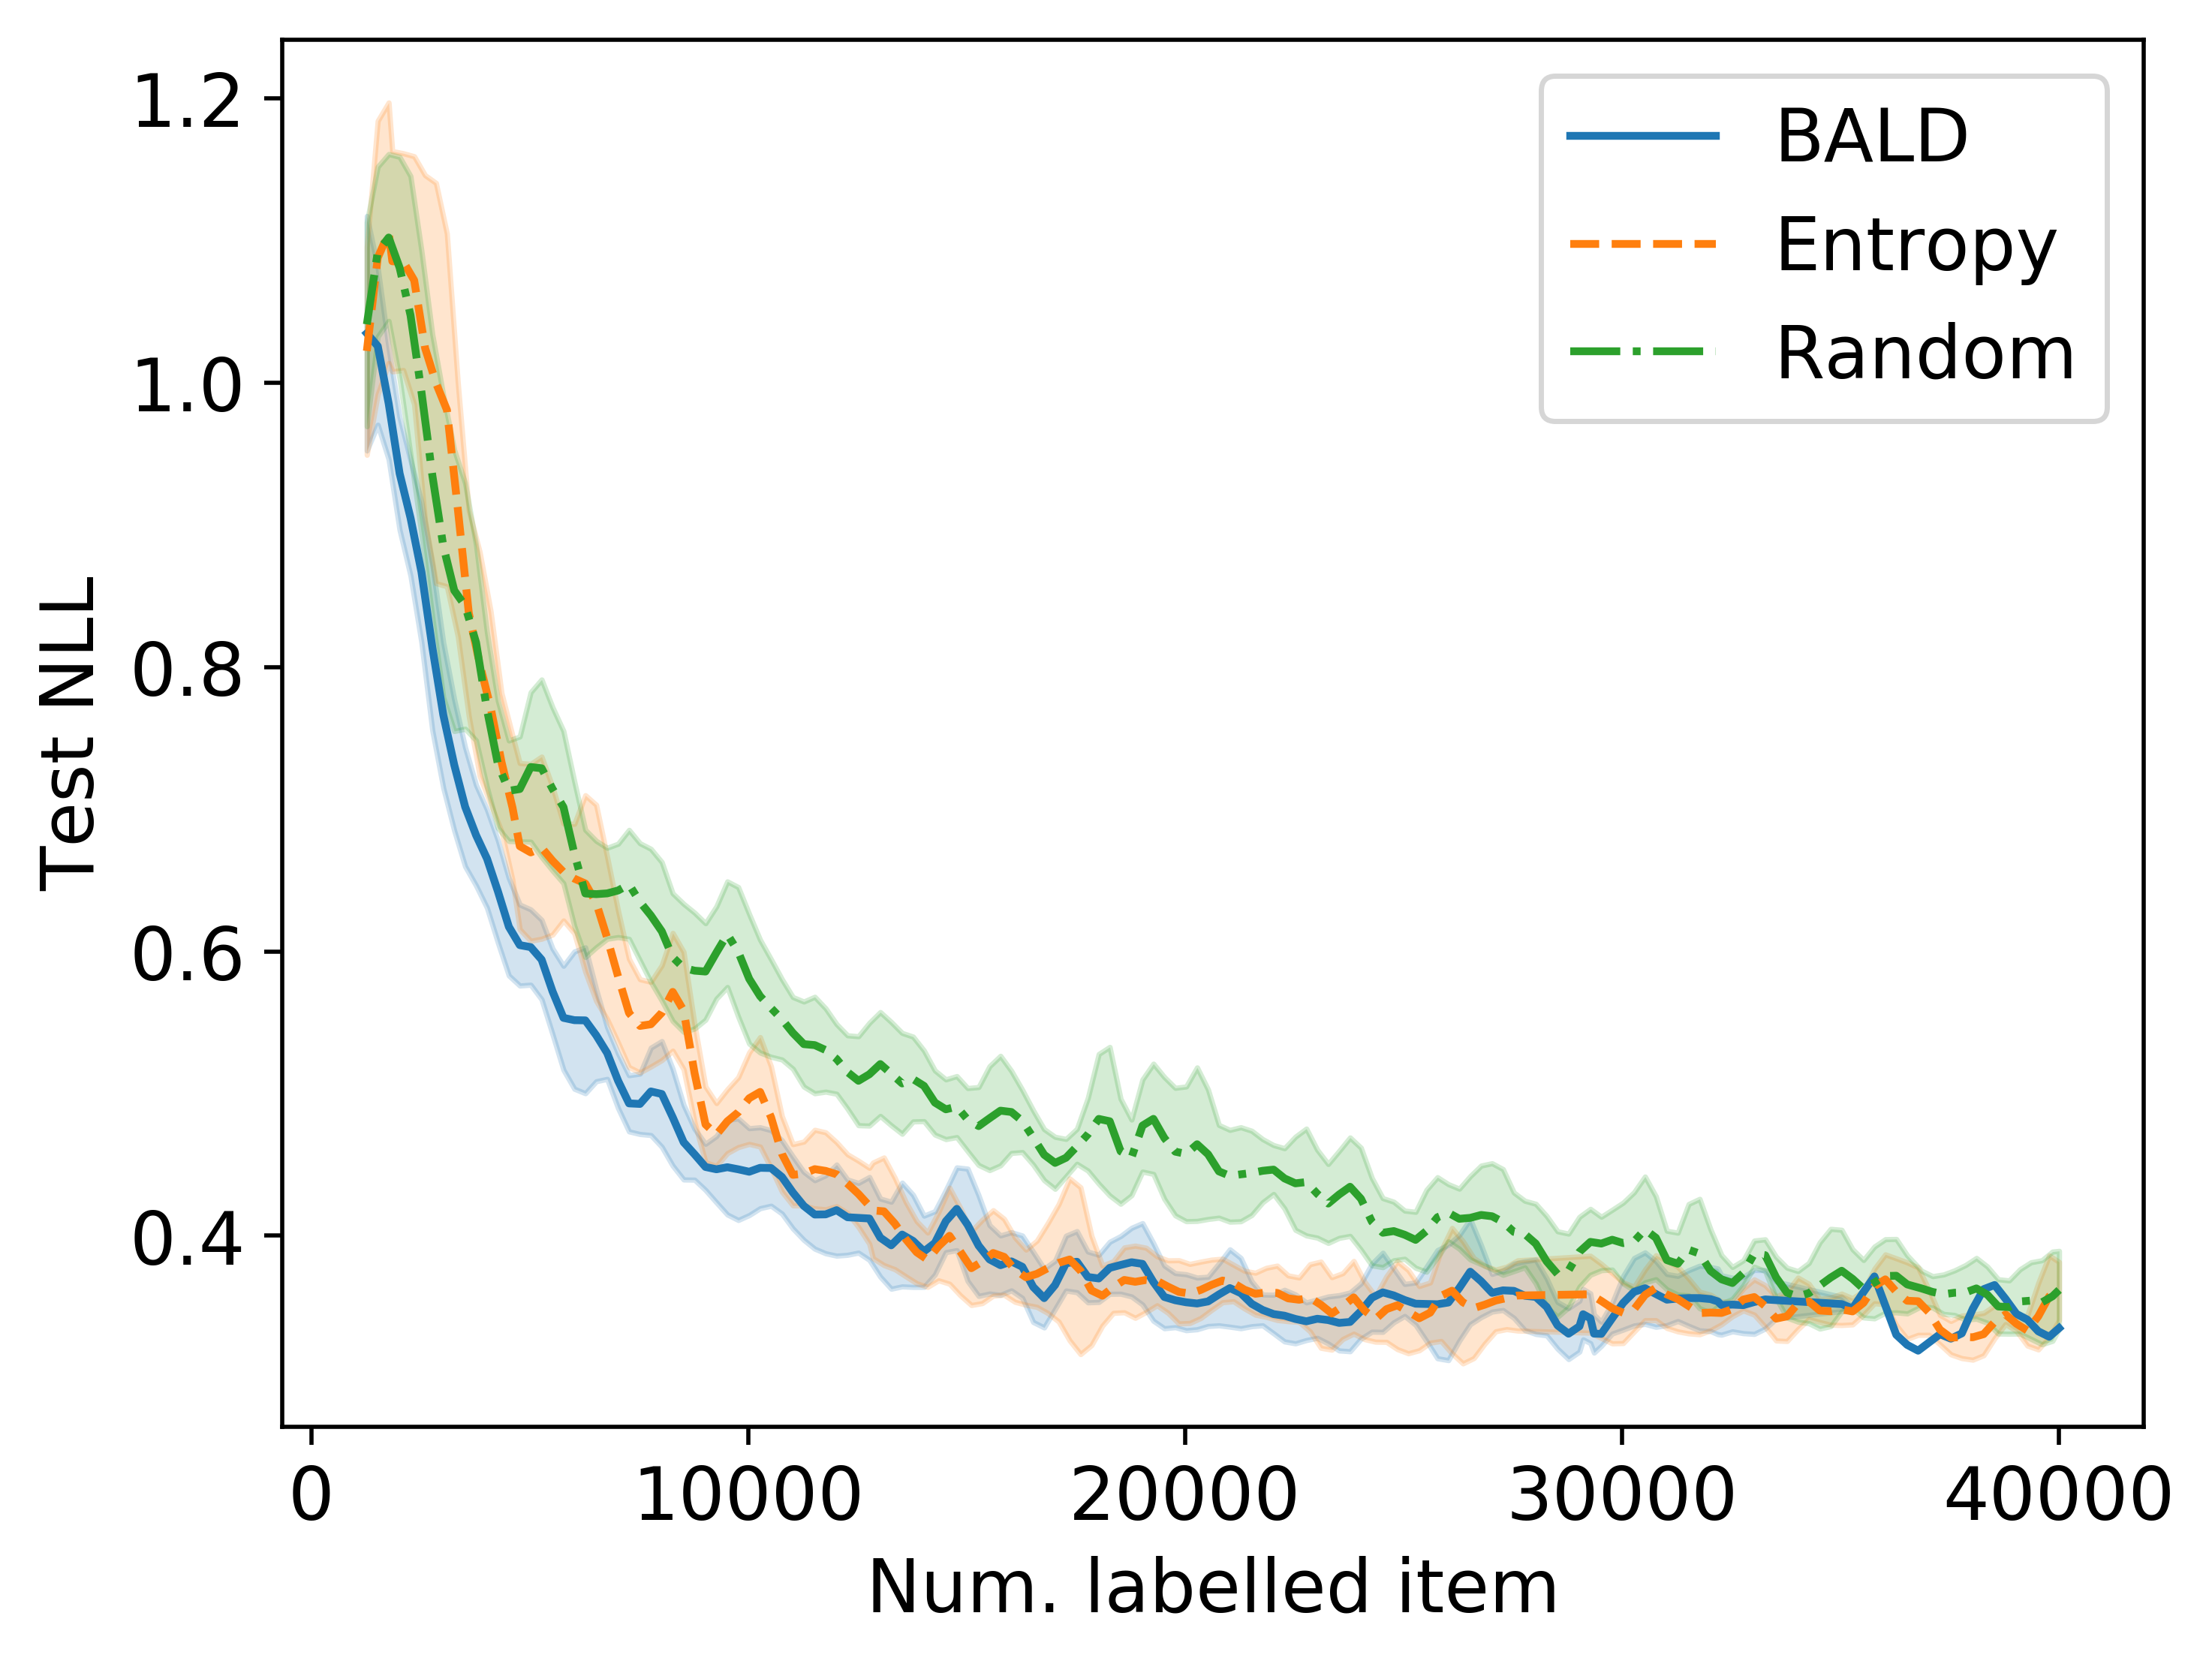
\includegraphics[width=0.4\textwidth]{fig/standard.png}
    \caption{Baselines results on CIFAR10 using MC-Dropout and VGG-16. On an academic dataset, both active learning techniques are competitive.}
    \label{fig:standard}
\end{figure}

\begin{abstract}
\vspace{-0.60cm}
   Active learning is able to reduce the amount of labelling effort by using a machine learning model to query the user for specific inputs.
   While there are many papers on new active learning techniques, these techniques rarely satisfy the constraints of a real-world project. In this paper, we analyse the main drawbacks of current active learning techniques and we present approaches to alleviate them. We do a systematic study on the effects of the most common issues of real-world datasets on the deep active learning process: model convergence, annotation error, and dataset imbalance. We derive two techniques that can speed up the active learning loop such as partial uncertainty sampling and larger query size. Finally, we present our open-source Bayesian active learning library, BaaL.
\end{abstract}

\bibliography{example_paper}
\bibliographystyle{icml2020}
% For submission, needs to be 2 documents and then concat together.
\end{document}



% This document was modified from the file originally made available by
% Pat Langley and Andrea Danyluk for ICML-2K. This version was created
% by Iain Murray in 2018, and modified by Alexandre Bouchard in
% 2019 and 2020. Previous contributors include Dan Roy, Lise Getoor and Tobias
% Scheffer, which was slightly modified from the 2010 version by
% Thorsten Joachims & Johannes Fuernkranz, slightly modified from the
% 2009 version by Kiri Wagstaff and Sam Roweis's 2008 version, which is
% slightly modified from Prasad Tadepalli's 2007 version which is a
% lightly changed version of the previous year's version by Andrew
% Moore, which was in turn edited from those of Kristian Kersting and
% Codrina Lauth. Alex Smola contributed to the algorithmic style files.
